% ======================================================================
% CVPR 2026 Workshop: Foundation Models for Medical Vision
% Challenge: Foundation Models for General CT Image Diagnosis
% Task 1 (Linear Probing) -- All Data Track
% Team: maest   |   Method: MAE-ST (video-style spatiotemporal MAE for CT;
%                            forked from facebookresearch/mae_st)
% ----------------------------------------------------------------------
% NOTE TO AUTHORS: cells marked \tba{} need a final value or check before
% camera-ready. See NOTES_FOR_AUTHORS.md for the full list.
% ======================================================================
\documentclass[runningheads]{llncs}

\usepackage[T1]{fontenc}
\usepackage{multirow}
\usepackage{graphicx}
\usepackage{booktabs}
\usepackage{xcolor}
\usepackage{amsmath}
\usepackage{tikz}
\usetikzlibrary{arrows.meta,positioning,fit,backgrounds,calc}
\usepackage[pagebackref=true,breaklinks=true,colorlinks,bookmarks=false]{hyperref}

% Placeholder marker for numbers still to be filled / verified.
\newcommand{\tba}{\textcolor{red}{\textbf{[TBD]}}}

\begin{document}

\title{Computed Tomography as Video: A Spatiotemporal Masked Autoencoder for Linear-Probe CT Diagnosis}
\titlerunning{CT-as-Video Spatiotemporal MAE for Linear-Probe Diagnosis}

\author{Gautham Nandakumar\inst{1}\orcidID{0000-0000-0000-0000}}
\authorrunning{G. Nandakumar}
\institute{Calico Life Sciences LLC, South San Francisco, CA, USA\\
\email{gautham@calicolabs.com}}

\maketitle

% ======================================================================
\begin{abstract}
We present \textbf{MAE-ST}, our submission to Task~1 (Linear Probing, LP)
\textbf{All-Data track} of the CVPR~2026 Challenge on Foundation Models for
General CT Image Diagnosis. Our method is forked from the official MAE-ST
codebase (\texttt{facebookresearch/mae\_st}) and adapted for single-channel CT
volumes. The central idea is to treat a 3D CT volume as a
short \emph{video}: the axial (Z) axis is interpreted as a temporal axis, and a
ViT-Large spatiotemporal masked autoencoder ($303.6$\,M parameters) is
pre-trained from scratch on $10{,}819$ unlabeled CT volumes drawn from the
challenge pre-training corpus. Two design choices drive the representation: a
\emph{dynamic} masking ratio sampled uniformly from $[0.6, 0.9]$ on every
forward pass, which exposes the encoder to a range of reconstruction
difficulties rather than a single fixed one, and a coarse
temporal patch size ($4$ slices) that concentrates capacity on in-plane
anatomy. At inference the encoder is \emph{frozen}: each volume is processed by
overlapping $16$-slice windows, and the layer-normalized mean of the patch
tokens is averaged across windows to yield a single $1024$-dimensional
descriptor; for the eleven region-of-interest (ROI) targets the descriptor is
restricted to the organ mask provided by the organizers. On our validation set
($15$ AMOS abdominal targets) the frozen features reach a \textbf{mean AUROC of
$0.678$}. On the final, held-out \emph{test} set
($17$ binary targets across three datasets) the same system scores a
\textbf{balanced accuracy of $0.600$ and an AUROC of $0.624$} at
\textbf{$6.27$\,s per case}, ranking $4^{\text{th}}$ on the
All-Data LP leaderboard. We additionally report a recipe-level ablation against
an ablated baseline. \\[4pt]
\keywords{CT foundation model \and Linear probing \and Masked autoencoder \and
Spatiotemporal modeling \and Binary classification.}
\end{abstract}

% ======================================================================
\section{Introduction}

Computed tomography (CT) is the workhorse of cross-sectional diagnostic imaging,
and the past two years have produced a wave of CT \emph{foundation models} that
aim to provide a single reusable representation for many downstream diagnostic
tasks~\cite{voco,ctfm,merlin,ctclip,pillar0}. Despite this rapid progress, two
difficulties persist, and they are precisely the ones this challenge stresses.
The first is generalization across anatomy and acquisition: a representation
tuned on one body region or one scanner population frequently degrades on
another, and the challenge deliberately spans abdomen and chest across multiple
source datasets. The second is severe class imbalance, since the downstream
targets are binary disease labels whose positive prevalence is often well below
$10\%$, so raw accuracy is uninformative and \emph{balanced accuracy} and AUROC
become the metrics of record.

Against this backdrop, we address \textbf{Task~1 -- Linear Probing (LP)} of the
challenge, in which the pre-trained backbone is kept \emph{frozen} and only a
lightweight linear classifier is trained on top of its features, with no
backbone fine-tuning. This setting isolates the intrinsic discriminative power
of a pre-trained representation: how well the features learned during
self-supervised pre-training transfer, on their own, to binary CT disease
classification. Our submission is built entirely for this Task~1 LP setting.

Prior work approaches CT representation learning from several directions that
differ mainly in their source of supervision. \emph{Vision-only} models learn
from image content alone. VoCo~\cite{voco} pre-trains a SwinUNETR with a
volume-contrastive objective that predicts the spatial overlap between cropped
sub-volumes, pulling anatomically aligned regions together in feature space;
CT-FM~\cite{ctfm} and the 3D framework of Xu~et~al.~\cite{ctfm_xu} scale
contrastive and reconstruction pretext tasks to large unlabeled CT collections;
and Curia~\cite{curia} consolidates many radiology sources into a single
multi-task backbone. \emph{Vision-language} models add free-text supervision:
Merlin~\cite{merlin}, CT-CLIP~\cite{ctclip}, and Pillar-0~\cite{pillar0} learn a
CLIP-style alignment between CT volumes and their radiology reports, which
enables zero-shot abnormality detection and stronger supervised transfer, while
the hybrid SPECTRE~\cite{SPECTRE} combines self-supervised reconstruction with
cross-modal alignment in a volumetric transformer.

Orthogonal to the supervisory signal is the choice of pretext mechanism and how
the resulting backbone is adapted. The masked autoencoder~\cite{mae} hides a
large fraction of image patches and reconstructs them with an asymmetric
encoder--decoder, learning representations without contrastive pairs or labels;
its spatiotemporal extension MAE-ST~\cite{maest} randomly masks a large fraction
of space--time patches so that a video encoder must infer the missing content
from the surrounding frames.
Once pre-trained, a backbone must be adapted to a downstream decision: linear
probing~\cite{linearprobing} trains only a linear classifier on frozen features
and therefore reports their intrinsic quality, whereas LoRA~\cite{lora} and
adapters~\cite{adapter} inject a small number of trainable parameters when the
backbone is allowed to move. Across these lines, the field is dominated by
contrastive or report-aligned objectives and by CNN/Swin backbones; the behavior
of a \emph{pure reconstructive ViT} that models the through-plane ($Z$) axis
explicitly, evaluated under a strict frozen-feature protocol, remains
comparatively unexplored.

This gap motivates our approach. A CT volume is, geometrically, a stack of axial
slices with strong continuity along Z -- exactly the structure that video
transformers exploit between frames. We therefore repurpose the spatiotemporal
masked autoencoder MAE-ST~\cite{maest} for CT, with the Z axis playing the role
of time. Our implementation is a direct fork of the official MAE-ST
codebase~\cite{maest}\footnote{\url{https://github.com/facebookresearch/mae_st}},
adapted for single-channel CT volumes. This buys us two things: a masked
reconstruction objective in which a large, randomly chosen fraction of
space-time patches is dropped, forcing the encoder to infer the occluded anatomy
from surrounding 3D context, and a ViT-Large backbone whose patch-token mean is a
strong frozen descriptor. Our contributions are:
\begin{enumerate}
  \item \textbf{A CT-adapted spatiotemporal MAE (MAE-ST)} pre-trained
        \emph{from scratch} on the full $10{,}819$-volume All-Data corpus, with
        two changes that matter empirically: a \emph{dynamic} mask ratio
        $\sim\mathcal{U}[0.6,0.9]$ (a range of reconstruction difficulties
        within one run) and a coarse temporal patch ($4$ slices).
  \item \textbf{A frozen feature-extraction recipe} for arbitrary-depth volumes:
        overlapping $16$-slice windows, layer-normalized token-mean pooling, and
        mask-guided ROI restriction for the eleven ROI targets -- all running at
        $6.27$\,s/case, comfortably within the $40$\,s budget.
  \item \textbf{An honest empirical study}: validation results ($0.678$ mean
        AUROC), the final test ranking ($4^{\text{th}}$ on the leaderboard,
        top six shown; $0.624$ AUROC,
        $0.600$ balanced accuracy), and a recipe-level ablation against an
        ablated baseline.
\end{enumerate}

% ======================================================================
\section{Method}

Figure~\ref{fig:Network} shows the full pipeline: (a) self-supervised
spatiotemporal MAE pre-training on unlabeled CT, and (b) frozen feature
extraction feeding the organizer-run linear probe.

\begin{figure}[t]
\centering
\resizebox{\textwidth}{!}{%
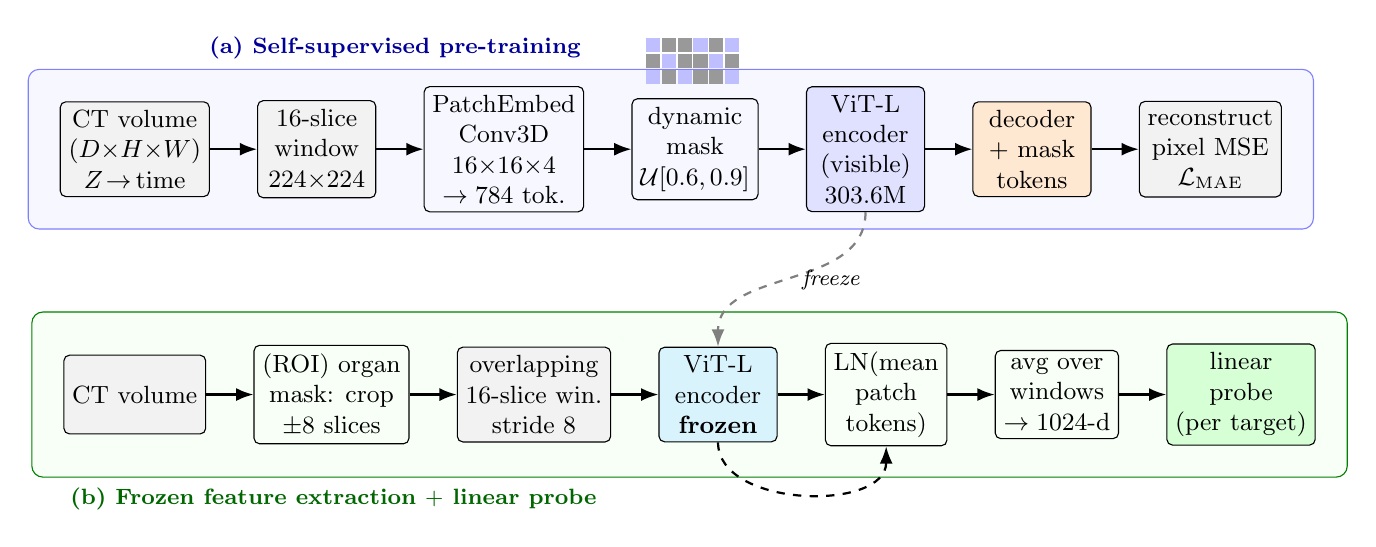
\begin{tikzpicture}[
  font=\small,
  >={Latex[length=2.2mm]},
  node distance=5.5mm and 6mm,
  block/.style={draw, rounded corners=2pt, align=center, minimum height=10mm,
                minimum width=15mm, inner sep=3pt},
  data/.style={block, fill=black!5},
  enc/.style={block, fill=blue!12},
  dec/.style={block, fill=orange!18},
  frozen/.style={block, fill=cyan!15},
  head/.style={block, fill=green!16},
  lbl/.style={font=\footnotesize\itshape},
  arr/.style={->, thick}
]

% ---------- Row (a): self-supervised pre-training ----------
\node[data] (vol) {CT volume\\$(D{\times}H{\times}W)$\\$Z\!\to\!$ time};
\node[data, right=of vol] (win) {$16$-slice\\window\\$224{\times}224$};
\node[block, right=of win] (pe) {PatchEmbed\\Conv3D\\$16{\times}16{\times}4$\\$\to 784$ tok.};
\node[block, right=of pe] (mask) {dynamic\\mask\\$\mathcal{U}[0.6,0.9]$};
\node[enc, right=of mask] (enc) {ViT-L\\encoder\\(visible)\\$303.6$M};
\node[dec, right=of enc] (dec) {decoder\\$+$ mask\\tokens};
\node[data, right=of dec] (rec) {reconstruct\\pixel MSE\\$\mathcal{L}_{\text{MAE}}$};

\draw[arr] (vol)--(win);
\draw[arr] (win)--(pe);
\draw[arr] (pe)--(mask);
\draw[arr] (mask)--(enc);
\draw[arr] (enc)--(dec);
\draw[arr] (dec)--(rec);

% small masked-token grid above the mask node (grey = masked, light = visible)
\begin{scope}[shift={($(mask.north)+(-0.62,0.18)$)}]
  \foreach \x in {0,...,5}{
    \foreach \y in {0,...,2}{
      \pgfmathtruncatemacro{\m}{mod(\x*2+\y*3+\x,5)>1 ? 1 : 0}
      \ifnum\m=1
        \fill[black!40] (\x*0.2,\y*0.2) rectangle ++(0.18,0.18);
      \else
        \fill[blue!25] (\x*0.2,\y*0.2) rectangle ++(0.18,0.18);
      \fi
    }
  }
\end{scope}

% ---------- Row (b): frozen feature extraction + linear probe ----------
\node[data, below=20mm of vol] (vol2) {CT volume};
\node[block, right=of vol2] (roi) {(ROI) organ\\mask: crop\\$\pm8$ slices};
\node[data, right=of roi] (winN) {overlapping\\$16$-slice win.\\stride $8$};
\node[frozen, right=of winN] (enc2) {ViT-L\\encoder\\\textbf{frozen}};
\node[block, right=of enc2] (pool) {LN(mean\\patch\\tokens)};
\node[block, right=of pool] (avg) {avg over\\windows\\$\to 1024$-d};
\node[head, right=of avg] (lp) {linear\\probe\\(per target)};

\draw[arr] (vol2)--(roi);
\draw[arr] (roi)--(winN);
\draw[arr] (winN)--(enc2);
\draw[arr] (enc2)--(pool);
\draw[arr] (pool)--(avg);
\draw[arr] (avg)--(lp);
% feedback that each window is encoded then pooled
\draw[arr, dashed] (enc2.south) to[out=-90,in=-90] (pool.south);

% reuse of pretrained weights: encoder (a) -> frozen encoder (b)
\draw[->, thick, dashed, gray] (enc.south) to[out=-90,in=90]
      node[midway,right,lbl,black]{freeze} (enc2.north);

% ---------- background panels with stage labels ----------
\begin{scope}[on background layer]
  \node[draw=blue!50, rounded corners, fill=blue!3, inner sep=4mm,
        fit=(vol)(rec), label={[font=\bfseries\footnotesize,blue!60!black]
        above left:(a) Self-supervised pre-training}] {};
  \node[draw=green!50!black, rounded corners, fill=green!3, inner sep=4mm,
        fit=(vol2)(lp), label={[font=\bfseries\footnotesize,green!40!black]
        below left:(b) Frozen feature extraction $+$ linear probe}] {};
\end{scope}

\end{tikzpicture}%
}
\caption{Pipeline. \textbf{(a) Pre-training:} a CT volume is treated as a video
($Z\!\to\!$ time); a random $16$-slice window at $224^2$ is patch-embedded with a
$16{\times}16$ spatial / $4$-slice temporal kernel into $4{\times}14{\times}14{=}784$
tokens, a dynamic fraction ($60$--$90\%$, grey squares) is masked, the ViT-Large
encoder sees only the visible tokens (blue squares), and a lightweight decoder
reconstructs the masked voxels under a pixel-MSE loss. \textbf{(b) Feature
extraction (frozen):} the trained encoder is frozen; a volume is tiled into
overlapping $16$-slice windows (stride $8$), each window yields a
layer-normalized patch-token mean, and the per-window vectors are averaged into a
single $1024$-d descriptor on which the organizers train a linear probe. For the
eleven ROI targets the volume is first cropped to the provided organ mask
($\pm8$ context slices).}
\label{fig:Network}
\end{figure}

\subsection{Self-supervised pre-training}

\paragraph{CT-as-video formulation.}
A CT volume of shape $(D,H,W)$ is normalized (Sec.~\ref{sec:preproc}) and a
contiguous window of $T{=}16$ axial slices is resized to $16{\times}224{\times}224$
and treated as a single-channel ($C{=}1$) clip. A 3D patch-embedding convolution
with spatial kernel $16{\times}16$ and \emph{temporal kernel $4$} (stride equal
to kernel) produces a token grid of size $(T/4)\times(H/16)\times(W/16)=
4{\times}14{\times}14=784$ tokens of dimension $1024$, to which a learnable
class token and \emph{separable} spatial/temporal positional embeddings are
added.

\paragraph{Masked reconstruction.}
Following MAE~\cite{mae,maest}, on each forward pass we sample a masking ratio
$r\sim\mathcal{U}[0.6,0.9]$ and randomly drop a fraction $r$ of the $784$ tokens.
The ViT-Large \emph{encoder} ($24$ blocks, $1024$-d, $16$ heads,
mlp-ratio $4$) processes only the visible tokens. An asymmetric
\emph{decoder} ($8$ blocks, $512$-d, $16$ heads) receives the encoded visible
tokens plus shared mask tokens and reconstructs the masked content; the loss is
the mean-squared error between predicted and ground-truth voxels, computed
\emph{only over masked patches} (raw-pixel target, no per-patch normalization):
\[
\mathcal{L}_{\text{MAE}}
= \frac{1}{|\mathcal{M}|}\sum_{i\in\mathcal{M}}\big\lVert \hat{x}_i - x_i \big\rVert_2^2 ,
\]
where $\mathcal{M}$ indexes masked patches. The temporal prediction dimension is
$16$, so the decoder reconstructs all $16$ input slices.

\paragraph{Why dynamic masking.}
A fixed high ratio (e.g.\ $90\%$) leaves only $\sim\!157$ visible
tokens and makes \emph{every} iteration maximally hard. Sampling
$r\sim\mathcal{U}[0.6,0.9]$ independently each step instead exposes the encoder
to a range of reconstruction difficulties -- from $\sim\!627$ visible tokens
($60\%$, rich context) to $\sim\!157$ ($90\%$, aggressive inpainting) -- within a
single training run, rather than committing to one fixed difficulty. The
sampling distribution is stationary across training, so this is difficulty
\emph{mixing} rather than a scheduled easy-to-hard curriculum. This is
consistent with recent evidence that exposing a masked autoencoder to a
\emph{range} of masking ratios, rather than a single fixed value, encourages
multi-scale feature learning and can surpass even the best-tuned fixed
ratio~\cite{r2mae}. We expect it to be a major contributor to feature quality;
rigorous isolation against the other six changes is left for future work
(Sec.~\ref{sec:ablation}).

\paragraph{Backbone details.}
ViT-Large, patch $16{\times}16$ (spatial) $\times\,4$ (temporal), embedding
dimension $1024$, depth $24$, $16$ heads, mlp-ratio $4$, separable
spatio-temporal position embeddings and a class token. The frozen encoder loaded
at inference has \textbf{$303.6$\,M parameters} (decoder and mask tokens are
stripped from the checkpoint and are not shipped in the container).

\subsection{Inference: frozen feature extraction and linear probing}
\label{sec:inference}
At inference the decoder is discarded and the encoder is frozen; the system maps
a full-resolution, arbitrary-depth CT volume to a single descriptor that the
organizers' linear probe then classifies.

\paragraph{Global feature from the frozen backbone.}
Given a single $16$-slice
window, we run the frozen encoder \emph{without} masking, drop the class token, take the
\emph{mean over the $784$ patch tokens}, and apply the final encoder
LayerNorm, yielding a $1024$-d vector. We chose mean-pooled patch tokens over the
class token because, under a reconstructive objective, the class token is never
supervised, whereas patch tokens directly carry localized anatomical evidence.

\paragraph{Windowed aggregation for arbitrary-depth volumes.}
\label{sec:agg}
Clinical CTs have variable depth $D$ (tens to hundreds of slices), but the
encoder consumes exactly $16$ slices. We therefore slide a $16$-slice window
along Z with \textbf{stride $8$ ($50\%$ overlap)}, resize each window in-plane to
$224^2$ by trilinear interpolation, and \emph{average} the per-window $1024$-d
descriptors into one volume-level vector. A final window anchored at the last
slice guarantees full Z coverage when $D$ is not a multiple of the stride.
Overlapping windows make the descriptor robust to where structures fall relative
to window boundaries. Rather than encoding one window at a time, we stack $8$
windows into a single GPU batch, which uses the device far more efficiently and
speeds up per-case feature extraction.

\paragraph{ROI versus non-ROI targets.}
Eleven targets are ROI-based (organ-specific): for these the organizers provide a
foreground organ mask, and we restrict feature extraction to the masked
sub-volume; the remaining targets are treated globally (whole-volume descriptor).
For an ROI target we read the provided mask, find the Z-range where the mask is
active, expand it by $\pm 8$ context slices, crop the volume to that range, and
then apply the same windowed aggregation. This focuses the descriptor on the
organ of interest (e.g.\ adrenal gland for \emph{adrenal\_hyperplasia}) while
retaining peri-organ context. Cropping also leaves fewer $16$-slice windows to
pass through the ViT, which lowers per-case compute and runtime. If a mask is
empty we fall back to the global descriptor.

\paragraph{Linear-probe head.}
The container emits only frozen $1024$-d features; per challenge protocol, the
\emph{organizers} fit the linear probe. For internal model selection we
replicate the standard LP recipe: $L_2$-normalize each descriptor and fit a
per-target $\ell_2$-regularized logistic regression with
\emph{class-balanced} weighting (to counter the severe positive/negative
imbalance), sweeping the inverse regularization strength
$C\in\{10^{-3},10^{-2},10^{-1},1,10,10^{2}\}$ and selecting by validation AUROC.
A linear probe has no capacity to compensate for a weak backbone, which is
exactly why it is a faithful probe of feature quality.

% ======================================================================
\section{Experiments}

\subsection{Dataset and evaluation metrics}
The challenge provides a large-scale unlabeled CT pre-training set and a
downstream train/validation set of \textbf{$17$ binary classification targets
across three datasets}, spanning abdomen and chest. For Task~1 we enter the
\textbf{All-Data track}, pre-training from scratch on the full corpus. Our
\emph{internal} validation pipeline covers the $15$ abdominal (AMOS-derived)
targets -- $11$ ROI and $4$ non-ROI; the two additional official targets are
chest findings (a COVID-CT target and a lung-nodule-malignancy target) that are
absent from our local split, so all internally reported per-disease numbers are
\emph{abdominal}.

\noindent\textbf{Classification metrics.}
\emph{Balanced accuracy} (mean of sensitivity and specificity), robust to
imbalance, and \emph{AUROC}. \textbf{Efficiency metric:} per-case running time
in seconds, including container start-up; for Task~1 this is the average
feature-extraction time per target.

\subsection{Implementation details}

\subsubsection{Preprocessing.}
\label{sec:preproc}
Each NIfTI volume is loaded and transposed to $(D,H,W)$ with $Z$ first. Hounsfield
units are clipped to $[-1024, 3071]$ and linearly mapped to $[0,1]$; this single
fixed window is used at both pre-training and inference, so train/test
preprocessing is identical. During pre-training a random contiguous $16$-slice
window is drawn (short volumes are tiled to reach $16$ slices) and resized
in-plane to $224^2$ by trilinear interpolation. At inference the deterministic
overlapping-window scheme of Sec.~\ref{sec:agg} replaces the random crop. For
fast large-scale loading we read NIfTI arrays lazily via memory-mapped
\texttt{dataobj} access and apply all augmentation on the fly on $(1,T,H,W)$
tensors; no resampling to isotropic spacing is performed, which avoids an
expensive global resample on every volume.

\subsubsection{Environment settings.}
Development and runtime environments are summarized in Table~\ref{table:env}.

\begin{table}[!htbp]
\caption{Development environments and requirements.}\label{table:env}
\centering
\begin{tabular}{ll}
\hline
System            & Ubuntu 20.04 LTS (kernel 5.4.0) \\ \hline
CPU               & Intel Xeon Gold 6130 @ $2.10$\,GHz ($2{\times}16$ cores, $64$ threads) \\ \hline
RAM (pre-training)& $96$\,GB (Slurm allocation) \\ \hline
RAM (inference)   & container limit $32$\,GB (\texttt{-m 32G}) \\ \hline
GPU (pre-training)& $3\times$ NVIDIA Titan RTX $24$\,GB \\ \hline
GPU (inference)   & $1\times$ NVIDIA GPU (\texttt{--gpus device=0}) \\ \hline
CUDA version      & $12.1$ \\ \hline
Programming language & Python $3.9$ \\ \hline
Deep learning framework & PyTorch $2.1.0$ \\ \hline
Key libraries     & nibabel, h5py, timm, iopath, numpy \\ \hline
\end{tabular}
\end{table}

\subsubsection{Training protocols.}
\textbf{(1) Data augmentation.} During pre-training, augmentations are applied
consistently across all $16$ slices of a clip: random horizontal flip ($p{=}0.5$),
vertical flip ($p{=}0.5$), random $90/180/270^{\circ}$ axial rotation, random
intensity scale $\mathcal{U}[0.95,1.05]$ and shift $\mathcal{U}[-0.05,0.05]$, and
additive Gaussian noise ($p{=}0.3$, $\sigma{=}0.02$), with values re-clamped to
$[0,1]$. Inference uses no augmentation (no test-time augmentation).
\textbf{(2) Sampling.} Each epoch draws one random $16$-slice window per volume
(random start index), giving stochastic depth coverage across epochs.
Repeat-augmentation ($\times4$) replicates each sampled clip into four
independently augmented views per iteration, so an optimizer step sees $96$
augmented samples spanning the $24$ unique clips of the effective batch.
\textbf{(3) Model selection.} We extract features at candidate checkpoints
(epochs $40$ and $130$) and select by internal validation mean AUROC; epoch
$130$ was submitted.

Table~\ref{table:training-lp} gives the full pre-training and linear-head
protocol.
Figure~\ref{fig:curve} shows the pre-training reconstruction loss and learning-rate
schedule: the masked-patch MSE drops sharply within the first few epochs and then
decreases smoothly, while the learning rate follows the $40$-epoch linear warm-up
to $9.4\times10^{-5}$ and the subsequent cosine decay. The submitted checkpoint
(epoch $130$) sits on the converged plateau.

\begin{figure}[htbp]
\centering
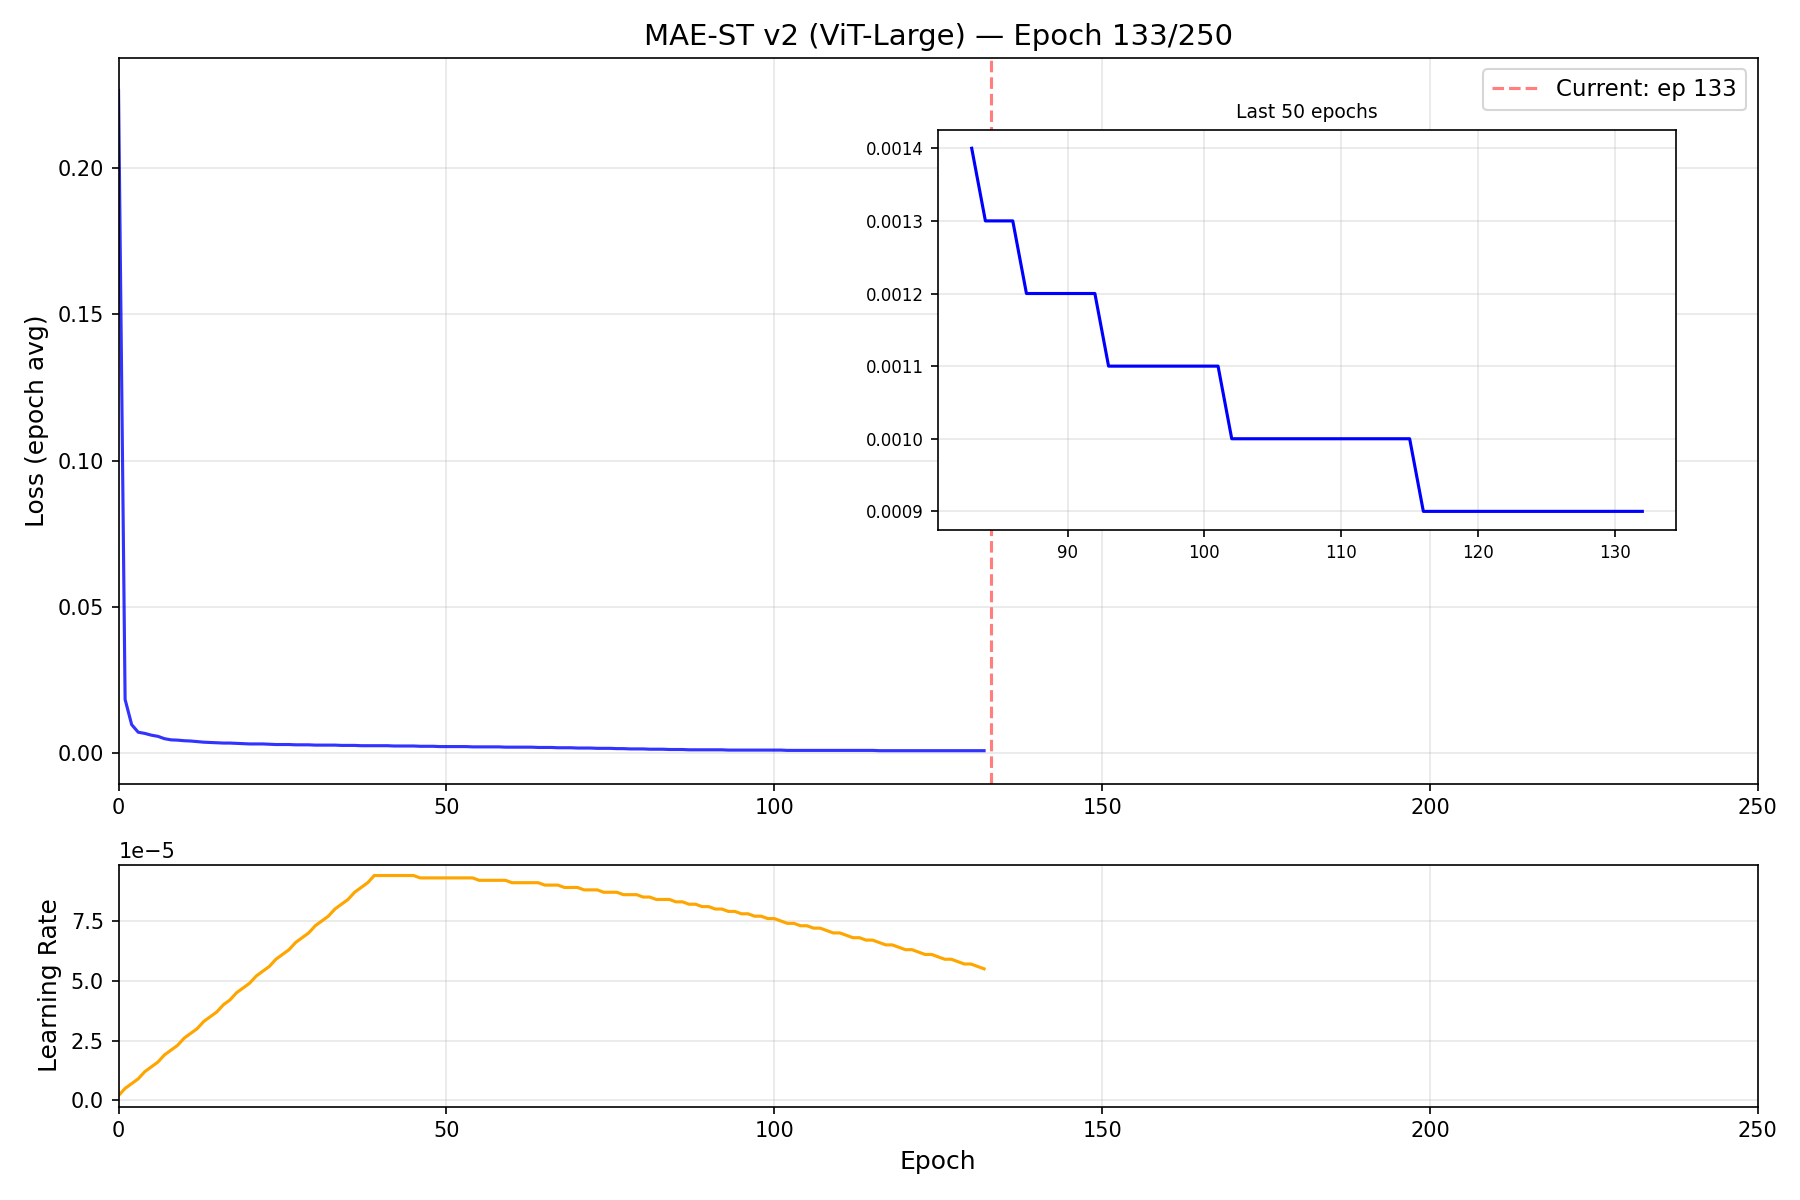
\includegraphics[width=\textwidth]{imgs/maest_training_curve.png}
\caption{MAE-ST (ViT-Large) pre-training. \textbf{Top:} per-epoch masked-patch
reconstruction loss (inset: last $50$ epochs, $\sim\!9\times10^{-4}$); the dashed
line marks the submitted epoch-$130$ checkpoint. \textbf{Bottom:} the per-epoch
learning rate -- linear warm-up over $40$ epochs to $9.4\times10^{-5}$ followed by
cosine decay (linear-scaling rule, effective batch $24$). Training ran to
epoch $133$ of $250$ scheduled and was stopped on the converged plateau; axes
are cropped to the trained range.}
\label{fig:curve}
\end{figure}

\begin{table*}[!htbp]
\caption{Training protocols for Task~1 -- Linear Probing (pre-training and
linear-head training).}
\label{table:training-lp}
\begin{center}
\begin{tabular}{ll}
\hline
Pre-trained backbone (if any)   & None -- MAE-ST pre-trained from scratch (All-Data) \\ \hline
Backbone tuning strategy        & Frozen \\ \hline
Batch size (pre-training)       & $24$ effective ($4$/GPU $\times\,2$ accum $\times\,3$ GPU) \\ \hline
Patch / volume size             & input $16\times224\times224$; patch $16\times16\times4$ \\ \hline
Total pre-training epochs       & $250$ scheduled; epoch $130$ submitted \\ \hline
Linear-head epochs              & Logistic regression, $C$-sweep (6 values), no SGD epochs \\ \hline
Optimizer                       & AdamW ($\beta=0.9,0.95$), weight decay $0.05$ \\ \hline
Initial learning rate (lr)      & $9.4\times10^{-5}$ (blr $10^{-3}\times24/256$) \\ \hline
Lr decay schedule               & Cosine to $0$, $40$-epoch linear warmup \\ \hline
Pre-training time               & $\approx 65.8$ hours ($1$ node, $3\times$ Titan RTX) \\ \hline
Linear-head training time       & $<1$ min/target (logistic regression) \\ \hline
Loss function                   & Masked-patch pixel MSE \\ \hline
Number of model parameters      & $303.6$\,M (frozen encoder) \\ \hline
\end{tabular}
\end{center}
\end{table*}

\subsection{Quantitative results on the validation set}

\paragraph{Validation performance.}
Under the frozen-LP protocol, MAE-ST attains a validation \textbf{mean AUROC of
$0.678$} (mean balanced accuracy $0.638$) over the $15$ AMOS abdominal targets.
This is higher than the $17$-target \emph{test} AUROC ($0.624$,
Sec.~\ref{sec:test}) because the official test set additionally averages in two
chest findings (COVID, lung-nodule malignancy) that are absent from our internal
validation split.

\paragraph{Per-disease validation detail.}
Table~\ref{tab:results-lp} reports per-target AUROC and balanced accuracy on the
class-balanced AMOS-15 validation set (epoch-130 submitted checkpoint). The
per-target dynamic range is large ($0.587\!\to\!0.841$ AUROC), which the mean
hides: the strongest targets are organ-scale, high-contrast findings
(splenomegaly, fatty liver), while the weakest are focal/cystic findings
(liver cyst, liver calcifications, gallstone). Aggregated by region of interest,
ROI and non-ROI targets are nearly tied ($0.685$ vs.\ $0.660$ mean AUROC).

\begin{table}[htbp]
\caption{Task~1 LP \textbf{All-Data}, \textbf{validation set}. Per-disease AUROC
and balanced accuracy on the class-balanced AMOS-15 internal validation split
(MAE-ST, epoch-130 submitted checkpoint; $303.6$\,M params). Targets sorted by
AUROC; $n_\text{val}$ is the number of balanced validation cases.}
\label{tab:results-lp}
\centering
\begin{tabular}{llccc}
\hline
Target & Type & AUROC & BalAcc & $n_\text{val}$ \\ \hline
splenomegaly         & ROI     & \textbf{0.841} & 0.729 & 70  \\ \hline
fatty\_liver          & ROI     & 0.825 & 0.679 & 78  \\ \hline
cholecystitis        & ROI     & 0.727 & 0.706 & 102 \\ \hline
adrenal\_hyperplasia  & ROI     & 0.713 & 0.686 & 70  \\ \hline
colorectal\_cancer    & non-ROI & 0.695 & 0.673 & 52  \\ \hline
hydronephrosis       & ROI     & 0.692 & 0.703 & 64  \\ \hline
lymphadenopathy      & non-ROI & 0.677 & 0.625 & 72  \\ \hline
kidney\_stone         & ROI     & 0.676 & 0.633 & 158 \\ \hline
ascites              & non-ROI & 0.655 & 0.647 & 68  \\ \hline
renal\_cyst           & ROI     & 0.639 & 0.605 & 266 \\ \hline
liver\_lesion         & ROI     & 0.620 & 0.522 & 134 \\ \hline
atherosclerosis      & non-ROI & 0.612 & 0.603 & 68  \\ \hline
gallstone            & ROI     & 0.607 & 0.612 & 116 \\ \hline
liver\_calcifications & ROI     & 0.603 & 0.569 & 72  \\ \hline
liver\_cyst           & ROI     & 0.587 & 0.578 & 244 \\ \hline
\textbf{All AMOS-15}  &         & \textbf{0.678} & \textbf{0.638} & 15 \\ \hline
ROI ($11$)           &         & 0.685 & 0.638 & 11 \\ \hline
non-ROI ($4$)        &         & 0.660 & 0.637 & 4  \\ \hline
\end{tabular}
\end{table}

\subsection{Ablation study}
\label{sec:ablation}

\paragraph{Submitted recipe vs.\ baseline.}
Table~\ref{tab:ablation} compares the submitted MAE-ST recipe against an
ablated baseline that differs in nine training choices simultaneously
(dynamic vs.\ fixed $90\%$ mask, raw-pixel vs.\ per-patch-normalized
reconstruction target, coarse vs.\ fine temporal patch, decoder depth,
repeated augmentation, base learning rate, gradient clipping,
warmup/training length, and an expanded augmentation pipeline). The full
recipe gains $+0.051$ AUROC ($0.627 \to 0.678$),
improving $12$ of $15$ targets. The largest per-target gains are on
organ-scale findings: splenomegaly $0.663\!\to\!0.841$ ($+0.178$),
liver calcifications $0.440\!\to\!0.603$ ($+0.163$, rescued from
below chance), and atherosclerosis $0.493\!\to\!0.612$ ($+0.119$, raised
above chance). Because the two configurations differ on nine
axes, we cannot isolate the contribution of any single change from this
comparison; per-axis attribution -- in particular for dynamic masking and
the raw-pixel loss target, which we expect to be major drivers -- is left
for follow-up work.

\begin{table}[htbp]
\caption{Ablation: submitted MAE-ST recipe vs.\ an ablated baseline (AMOS-15
internal validation, mean AUROC). The two configurations differ in nine
training choices listed below; per-design-choice attribution requires further
runs (Sec.~\ref{sec:limitations}).}\label{tab:ablation}
\centering
\begin{tabular}{lc}
\hline
Configuration & Mean AUROC \\ \hline
Ablated baseline & 0.627 \\
\textbf{MAE-ST submitted (ep130)} & \textbf{0.678} \\ \hline
\multicolumn{2}{l}{\footnotesize \textbf{Differences} (baseline $\rightarrow$
submitted):
mask $0.9 \to \mathcal{U}[0.6,0.9]$;} \\
\multicolumn{2}{l}{\footnotesize loss target per-patch-normalized $\to$ raw
pixels; $t_p\ 2 \to 4$; decoder depth $4 \to 8$;} \\
\multicolumn{2}{l}{\footnotesize repeat-aug $1 \to 4$;
blr $1.5{\times}10^{-4} \to 10^{-3}$; clip-grad $0.02 \to 1.0$;} \\
\multicolumn{2}{l}{\footnotesize warmup $10 \to 40$ ep; total $100 \to 250$ ep;
augmentation pipeline expanded.} \\ \hline
\end{tabular}
\end{table}

\paragraph{Aggregation and ROI cropping (design rationale).}
Two further design choices were guided by internal observations; we summarize
the rationale here.
\emph{(i) Multi-window overlap.} Overlapping ($50\%$) windows with mean pooling
were more stable than non-overlapping windows, particularly for findings that can
fall between window boundaries.
\emph{(ii) ROI cropping.} For the eleven ROI targets, mask-guided cropping
(organ range $\pm 8$ slices) concentrates the descriptor on the relevant organ
and reduces runtime by shrinking the window list. We did not run a head-to-head
comparison against whole-volume features, so we make no discrimination claim;
ROI and non-ROI targets in fact reach comparable validation AUROC
($0.685$ vs.\ $0.660$).

\subsection{Results on the final testing set}
\label{sec:test}
Table~\ref{tab:leaderboard} reports the official final-test ranking for the
Task~1 LP All-Data track. Our team (\textbf{maest}) places $4^{\text{th}}$ on the
published leaderboard (top six shown)
with $0.600$ balanced accuracy and $0.624$ AUROC at $6.27$\,s/case -- the
second-fastest runtime among the top four and roughly $5\times$ faster than the
slowest valid entry. The leading cluster (fomofo / raidium / cemrg) sits at
$0.705$--$0.714$ AUROC; we attribute most of the gap to cross-region (chest)
generalization (Sec.~\ref{sec:limitations}).

\begin{table}[htbp]
\caption{Official final-test ranking, Task~1 LP \textbf{All-Data} track ($17$
targets). Our submission is \textbf{maest}. Runtime is seconds per case including
container start-up.}\label{tab:leaderboard}
\centering
\begin{tabular}{clccc}
\hline
Rank & Team & Balanced Acc & AUROC & Runtime (s) \\ \hline
1 & fomofo            & 0.654 & 0.714 & 9.414 \\
1 & raidium           & 0.639 & 0.707 & 4.393 \\
3 & cemrg             & 0.643 & 0.705 & 4.467 \\
\textbf{4} & \textbf{maest (ours)} & \textbf{0.600} & \textbf{0.624} & \textbf{6.273} \\
5 & xupy              & 0.566 & 0.599 & 10.860 \\
6 & sdfmu             & 0.160 & 0.170 & 33.830 \\ \hline
\end{tabular}
\end{table}

\subsection{Limitations and future work}
\label{sec:limitations}
Our encoder is pre-trained on a predominantly
abdominal corpus and never sees the two chest targets in local validation;
closing the gap to the leaderboard leaders ($\sim\!0.09$ mean AUROC) likely
requires chest-CT pre-training data and region-balanced sampling. A single
mean-pooled descriptor is a strong but blunt
summary; attention pooling or multi-layer feature concatenation may recover
focal-lesion signal lost to averaging. We resize every volume to $224\times224$
in-plane and treat the $Z$ axis as time, discarding native pixel spacing in all
three axes; the model therefore never sees true physical scale. Spacing-aware
positional encodings or isotropic resampling that preserves the original $x$,
$y$, and $z$ resolution are natural extensions. Internal results are single-seed
on a small validation split;
multi-seed pre-training and bootstrap confidence intervals would tighten the
claims. Finally, our ablation contrasts the submitted recipe with
a single all-changes-flipped baseline; per-axis attribution requires
one-change-at-a-time runs that did not fit the challenge timeline.

% ======================================================================
\section{Conclusion}
We framed a 3D CT volume as a short video and pre-trained a spatiotemporal masked
autoencoder (MAE-ST, ViT-Large, $303.6$\,M parameters) from scratch on
$10{,}819$ unlabeled CT volumes for the All-Data linear-probing track. A dynamic
masking ratio and a coarse temporal patch yielded a frozen $1024$-d descriptor.
Via overlapping-window aggregation and mask-guided ROI cropping, this descriptor
achieved $0.678$ mean AUROC on our abdominal validation set and $0.600$ balanced
accuracy / $0.624$ AUROC at $6.27$\,s/case on the final test set, ranking
$4^{\text{th}}$ on the published All-Data LP leaderboard (top six shown). The main
lesson is methodological: a purely reconstructive ViT with explicit
through-plane modeling and a simple frozen-feature recipe is a competitive,
fast, and reproducible CT foundation-model baseline, whose principal remaining
weakness --- cross-region (chest) generalization --- chest-CT pre-training
should directly address.

\subsubsection{Acknowledgements.}
We thank the data owners for making the medical images publicly available and
Codabench~\cite{codabench} for hosting the challenge platform.

\subsubsection{Disclosure of Interests.}
The authors have no competing interests to declare that are relevant to the
content of this article.

\bibliographystyle{splncs04}
\bibliography{ref}

\end{document}
